\section{The Robot Software System (LabVIEW)}

\subsection{The Vehicle Co-Ordinate System}

The vehicle co-ordinate system is defined using the standard used on most ground vehicles: with the positive x direction straight ahead. In order to maintain a right-handed co-ordinate system, the three axes of the vehicle co-ordinate system are therefore defined as:

\begin{enumerate}
\item The positive X axis is pointed to the front of the vehicle
\item The positive Y axis is pointed to the left of the vehicle
\item The positive Z axis is pointed upward
\end{enumerate}

\noindent The respective rotations in the vehicle co-ordinate system are therefore defined as:

\begin{enumerate}
\item Positive rotation about the X axis (Positive Roll) is roll toward the driver's right side of the vehicle
\item Positive rotation about the Y axis (Positive Pitch) is pitch downward toward the ground
\item Positive rotation about the Z axis (Positive Yaw) is yaw toward the driver's left side (counter clockwise yaw) of the vehicle
\end{enumerate}

\subsection{LIDAR Point Transform}

The data returned by the Sick LMS290 LIDARs is in the co-ordinate frame of the LIDARs by virtue of the way in which the LIDARs take readings. In order to do useful work with the LIDAR data, the LIDAR data has to be transformed to make it iwth reference to the vehicle co-ordinate system. \\ \\
%
\noindent The transform process is essentially composed of 3 parts:

\begin{enumerate}
\item Flip the angle readings over since the LIDARs are upside down
\item Change the 0 degree position from the right most point to the point when the measurement is straight ahead
\item Add the counterclockwise rotation of the LIDAR units in the mount
\item 

\subsubsection{LIDAR Co-Ordinate Definition}
By default, the Sick LMS290 LIDARs are programmed to transmit distance measurements in millimeters (mm) and angles in degrees with 0 degrees on the right and 180 degrees on the left as shown in the image below:

\newpage
\begin{figure}[h!]
\centering
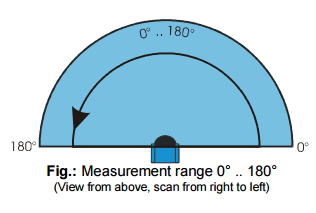
\includegraphics[scale=.8]{Photos/LIDAR_AngleDef.png}
\caption[Sick LMS290 Angle Definition]{Sick LMS290 Angle Definition \protect \footnotemark}
\label{fig:wholefish}
\end{figure} 
\footnotetext{ Information obtained from Quick Manula for LMS Communication Setup}

\subsubsection{Constant LIDAR Transform Properties}
Based on the design and placement of the LIDAR mounts, the following properties of the LIDAR transform to t